\documentclass[tikz]{standalone}

\usepackage{tikz}
\usetikzlibrary{decorations.pathreplacing}
\usetikzlibrary{positioning}\usepackage{etoolbox}

\begin{document}
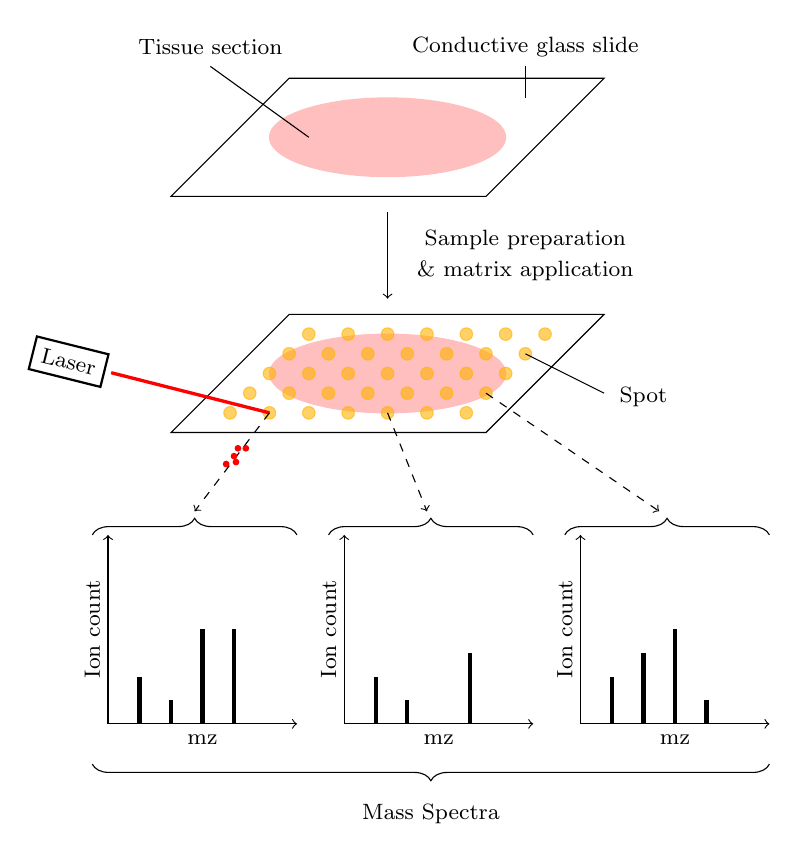
\begin{tikzpicture}
	
%	\draw (10.75,23.9) node {Mounted tissue section};
	\draw (8,22) -- (12,22) -- (13.5,23.5) -- (9.5,23.5) -- cycle;	
	
	\draw [fill = pink, draw = pink] (10.75,22.75) circle [x radius = 15mm, y radius = 5mm];
	
	\draw (8.5,23.9) node {\footnotesize Tissue section};
	\draw (9.75,22.75) -- (8.5,23.65);

	\draw (12.5,23.9) node {\footnotesize Conductive glass slide};
	\draw (12.5,23.25) -- (12.5,23.65);

	\draw [->] (10.75,21.8) -- (10.75,20.7);
	\draw (12.5,21.45) node {\footnotesize Sample preparation};
	\draw (12.5,21.05) node {\footnotesize \& matrix application};

	\draw (8,19) -- (12,19) -- (13.5,20.5) -- (9.5,20.5) -- cycle;	
	
	\draw [fill = pink, draw = pink] (10.75,19.75) circle [x radius = 15mm, y radius = 5mm];

	% Row 1
	\draw [fill = red!30!yellow, draw = red!30!yellow, opacity = 0.6] (8+0.25+0.5,19+0.25) circle [radius = 0.8mm];
	\draw [fill = red!30!yellow, draw = red!30!yellow, opacity = 0.6] (8+0.25+1.0,19+0.25) circle [radius = 0.8mm];
	\draw [fill = red!30!yellow, draw = red!30!yellow, opacity = 0.6] (8+0.25+1.5,19+0.25) circle [radius = 0.8mm];
	\draw [fill = red!30!yellow, draw = red!30!yellow, opacity = 0.6] (8+0.25+2.0,19+0.25) circle [radius = 0.8mm];
	\draw [fill = red!30!yellow, draw = red!30!yellow, opacity = 0.6] (8+0.25+2.5,19+0.25) circle [radius = 0.8mm];
	\draw [fill = red!30!yellow, draw = red!30!yellow, opacity = 0.6] (8+0.25+3.0,19+0.25) circle [radius = 0.8mm];
	\draw [fill = red!30!yellow, draw = red!30!yellow, opacity = 0.6] (8+0.25+3.5,19+0.25) circle [radius = 0.8mm];
	
	% Row 2	
	\draw [fill = red!30!yellow, draw = red!30!yellow, opacity = 0.6] (8+0.50+0.5,19+0.50) circle [radius = 0.8mm];
	\draw [fill = red!30!yellow, draw = red!30!yellow, opacity = 0.6] (8+0.50+1.0,19+0.50) circle [radius = 0.8mm];
	\draw [fill = red!30!yellow, draw = red!30!yellow, opacity = 0.6] (8+0.50+1.5,19+0.50) circle [radius = 0.8mm];
	\draw [fill = red!30!yellow, draw = red!30!yellow, opacity = 0.6] (8+0.50+2.0,19+0.50) circle [radius = 0.8mm];
	\draw [fill = red!30!yellow, draw = red!30!yellow, opacity = 0.6] (8+0.50+2.5,19+0.50) circle [radius = 0.8mm];
	\draw [fill = red!30!yellow, draw = red!30!yellow, opacity = 0.6] (8+0.50+3.0,19+0.50) circle [radius = 0.8mm];
	\draw [fill = red!30!yellow, draw = red!30!yellow, opacity = 0.6] (8+0.50+3.5,19+0.50) circle [radius = 0.8mm];

	% Row 3
	\draw [fill = red!30!yellow, draw = red!30!yellow, opacity = 0.6] (8+0.75+0.5,19+0.75) circle [radius = 0.8mm];
	\draw [fill = red!30!yellow, draw = red!30!yellow, opacity = 0.6] (8+0.75+1.0,19+0.75) circle [radius = 0.8mm];
	\draw [fill = red!30!yellow, draw = red!30!yellow, opacity = 0.6] (8+0.75+1.5,19+0.75) circle [radius = 0.8mm];
	\draw [fill = red!30!yellow, draw = red!30!yellow, opacity = 0.6] (8+0.75+2.0,19+0.75) circle [radius = 0.8mm];
	\draw [fill = red!30!yellow, draw = red!30!yellow, opacity = 0.6] (8+0.75+2.5,19+0.75) circle [radius = 0.8mm];
	\draw [fill = red!30!yellow, draw = red!30!yellow, opacity = 0.6] (8+0.75+3.0,19+0.75) circle [radius = 0.8mm];
	\draw [fill = red!30!yellow, draw = red!30!yellow, opacity = 0.6] (8+0.75+3.5,19+0.75) circle [radius = 0.8mm];
	
	% Row 4
	\draw [fill = red!30!yellow, draw = red!30!yellow, opacity = 0.6] (8+1.00+0.5,19+1.00) circle [radius = 0.8mm];
	\draw [fill = red!30!yellow, draw = red!30!yellow, opacity = 0.6] (8+1.00+1.0,19+1.00) circle [radius = 0.8mm];
	\draw [fill = red!30!yellow, draw = red!30!yellow, opacity = 0.6] (8+1.00+1.5,19+1.00) circle [radius = 0.8mm];
	\draw [fill = red!30!yellow, draw = red!30!yellow, opacity = 0.6] (8+1.00+2.0,19+1.00) circle [radius = 0.8mm];
	\draw [fill = red!30!yellow, draw = red!30!yellow, opacity = 0.6] (8+1.00+2.5,19+1.00) circle [radius = 0.8mm];
	\draw [fill = red!30!yellow, draw = red!30!yellow, opacity = 0.6] (8+1.00+3.0,19+1.00) circle [radius = 0.8mm];
	\draw [fill = red!30!yellow, draw = red!30!yellow, opacity = 0.6] (8+1.00+3.5,19+1.00) circle [radius = 0.8mm];

		% Row 5
		\draw [fill = red!30!yellow, draw = red!30!yellow, opacity = 0.6] (8+1.25+0.5,19+1.25) circle [radius = 0.8mm];
	\draw [fill = red!30!yellow, draw = red!30!yellow, opacity = 0.6] (8+1.25+1.0,19+1.25) circle [radius = 0.8mm];
	\draw [fill = red!30!yellow, draw = red!30!yellow, opacity = 0.6] (8+1.25+1.5,19+1.25) circle [radius = 0.8mm];
	\draw [fill = red!30!yellow, draw = red!30!yellow, opacity = 0.6] (8+1.25+2.0,19+1.25) circle [radius = 0.8mm];
	\draw [fill = red!30!yellow, draw = red!30!yellow, opacity = 0.6] (8+1.25+2.5,19+1.25) circle [radius = 0.8mm];
	\draw [fill = red!30!yellow, draw = red!30!yellow, opacity = 0.6] (8+1.25+3.0,19+1.25) circle [radius = 0.8mm];
	\draw [fill = red!30!yellow, draw = red!30!yellow, opacity = 0.6] (8+1.25+3.5,19+1.25) circle [radius = 0.8mm];

	\draw [very thick, draw = red] (7.24,19.76) -- (8+0.25+1.0,19+0.25);
	\node [draw, thick, rotate=346] at (6.7,19.9) {\footnotesize Laser};
		
	%mass spectra 1
	\draw [->,dashed] (8+0.25+1.0,19+0.25) -- (8.3,18);
	
	\draw [fill = red, draw = red] (8.8,18.7) circle [radius = 1pt];
	\draw [fill = red, draw = red] (8.95,18.8) circle [radius = 1pt];
	\draw [fill = red, draw = red] (8.85,18.8) circle [radius = 1pt];
	\draw [fill = red, draw = red] (8.7,18.6) circle [radius = 1pt];
	\draw [fill = red, draw = red] (8.825,18.625) circle [radius = 1pt];
	
	\node [draw = none, rotate=90] at (7,16.5) {{\footnotesize Ion count}};	
	\draw [->] (7.2,15.3) -- (7.2,17.7);
	\draw (8.4,15.1) node {{\footnotesize \gls{mz} }};
	\draw [->] (7.2,15.3) -- (9.6,15.3);
	\draw [ultra thick] (7.6,15.3) -- (7.6,15.3 + 0.6);
	\draw [ultra thick] (8,15.3) -- (8,15.3 + 0.3);
	\draw [ultra thick] (8.4,15.3) -- (8.4,15.3 + 1.2);
	\draw [ultra thick] (8.8,15.3) -- (8.8,15.3 + 1.2);
	\draw [decorate,decoration={brace,amplitude=6pt},yshift=0pt]
					(7,17.7) -- (9.6,17.7) node [black,midway,yshift=0pt] 
{};

	%mass spectra 2
	\draw [->,dashed] (8+0.25+2.5,19+0.25) -- (11.25,18);
	\node [draw = none, rotate=90] at (10,16.5) {{\footnotesize Ion count}};	
	\draw [->] (10.2,15.3) -- (10.2,17.7);
	\draw (11.4,15.1) node {{\footnotesize \gls{mz} }};
	\draw [->] (10.2,15.3) -- (12.6,15.3);
	\draw [ultra thick] (10.6,15.3) -- (10.6,15.3 + 0.6);
	\draw [ultra thick] (11,15.3) -- (11,15.3 + 0.3);
%	\draw [ultra thick] (11.4,15.3) -- (11.4,15.3 + 1.2);
	\draw [ultra thick] (11.8,15.3) -- (11.8,15.3 + 0.9);
	\draw [decorate,decoration={brace,amplitude=6pt},yshift=0pt]
					(10,17.7) -- (12.6,17.7) node [black,midway,yshift=0pt] 
{};
	
	%mass spectra 3
	\draw [->,dashed] (8+0.50+3.5,19+0.50) -- (14.2,18);
	\node [draw = none, rotate=90] at (13,16.5) {{\footnotesize Ion count}};	
	\draw [->] (13.2,15.3) -- (13.2,17.7);
	\draw (14.4,15.1) node {{\footnotesize \gls{mz} }};
	\draw [->] (13.2,15.3) -- (15.6,15.3);
	\draw [ultra thick] (13.6,15.3) -- (13.6,15.3 + 0.6);
	\draw [ultra thick] (14,15.3) -- (14,15.3 + 0.9);
	\draw [ultra thick] (14.4,15.3) -- (14.4,15.3 + 1.2);
	\draw [ultra thick] (14.8,15.3) -- (14.8,15.3 + 0.3);
	\draw [decorate,decoration={brace,amplitude=6pt},yshift=0pt]
					(13,17.7) -- (15.6,17.7) node [black,midway,yshift=0pt] 
{};
	
  % Spot annotation
  \draw (8+1.00+3.5,19+1.00) -- (8+1.00+3.5+1,19+1.00-0.5);
	\draw (8+1.00+3.5+1.5,19+1.00-0.55) node {\footnotesize Spot};
	
	
	\draw [decorate,decoration={brace,amplitude=6pt,mirror},yshift=-6pt]
					(7,15) -- (15.6,15) node [black,midway,yshift=-18pt] 
{\footnotesize Mass Spectra};



\end{tikzpicture}
\end{document}